\documentclass{article}
\usepackage{pgfplots}
\pgfplotsset{compat=1.16}
\usepackage{caption}

\begin{document}

\begin{figure}[h]
    \centering
    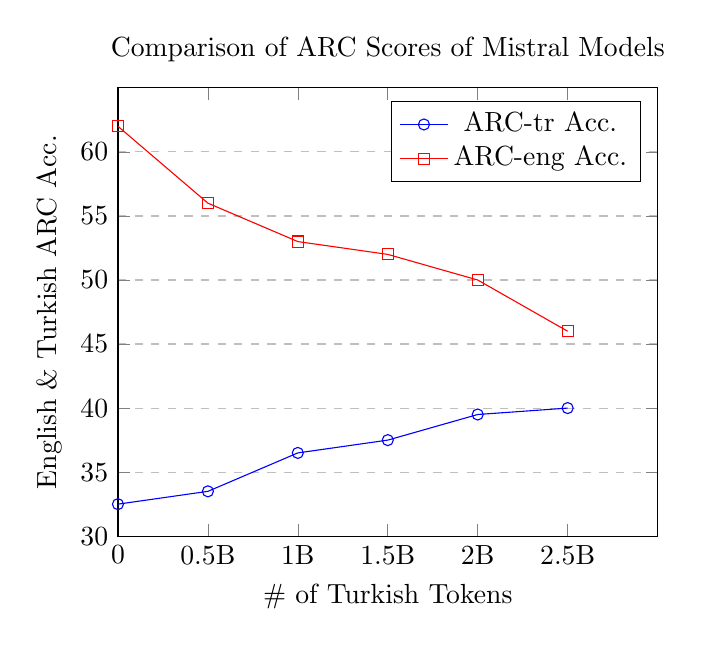
\begin{tikzpicture}
        \begin{axis}[
            title={Comparison of ARC Scores of Mistral Models},
            xlabel={\# of Turkish Tokens},
            ylabel={English \& Turkish ARC Acc.},
            xmin=0, xmax=3,
            ymin=30, ymax=65,
            xtick={0, 0.5, 1, 1.5, 2, 2.5},
            xticklabels={0, 0.5B, 1B, 1.5B, 2B, 2.5B},
            ytick={30, 35, 40, 45, 50, 55, 60},
            legend pos=north east,
            ymajorgrids=true,
            grid style=dashed,
        ]
        \addplot[
            color=blue,
            mark=o,
            ]
            coordinates {
                (0, 32.5)(0.5, 33.5)(1, 36.5)(1.5, 37.5)(2, 39.5)(2.5, 40)
            };
            \addlegendentry{ARC-tr Acc.}
        \addplot[
            color=red,
            mark=square,
            ]
            coordinates {
                (0, 62)(0.5, 56)(1, 53)(1.5, 52)(2, 50)(2.5, 46)
            };
            \addlegendentry{ARC-eng Acc.}
        \end{axis}
    \end{tikzpicture}
    \caption{Accuracy comparison of Continued Pretrained models on English (Left, Right) and Turkish (Right) question answering tasks and demonstrating the original language catastrophic forgetting while learning the new language. In the table on the left, the performance of our Hamza$_{\scriptsize Mistral}$ and Hamza$_{\scriptsize GPT2-xl}$ models that are adapted on Turkish together with the original Mistral 7B and GPT2-xl. We present the result of our ablation study, where the performance of the adapted models is given by progressively enlarging the pretraining corpus size from 0.1 GB to 5 GB. Here, the zero and few-show accuracies were evaluated on the original ARC and TruthfulQA. The figure on the right illustrates the Mistral model's results on both Turkish and English versions of the ARC dataset, highlighting its improved performance in Turkish and decreasing performance in English with continued pretraining.}
    \label{fig:arc_scores}
\end{figure}

\end{document}